By selecting e$^{+}$e$^{-}$ pairs from the triggered events we're able to study basic distributions related to our vertex performance. Pairs of opposite charge tracks, one in the top and one in the bottom half of the SVT, with larger than 400~MeV was selected. Figure~\ref{fig:vtx_pos} shows the distance of closest approach of the momentum vectors extrapolated in the upstream direction from our analyzing magnet, taking into account the measured fringe field. Relatively good agreement is found between data and an ideal simulation with the existing alignment of the SVT which provides confidence in our expected vertexing performance. The large distance to the converter and low statistics of the Test Run makes it hard to study the vertex resolution regime and tails of vertex distributions expected in the electron run. 
\begin{figure*}[t]
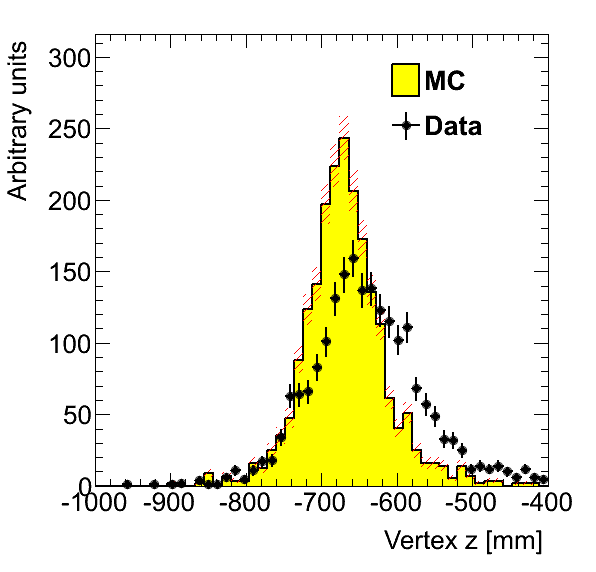
\includegraphics[ scale=0.25]{test2012/vertexing/figures/h_vtx_fr_x_h_vtx_x_dataMC_twotrksel.png}
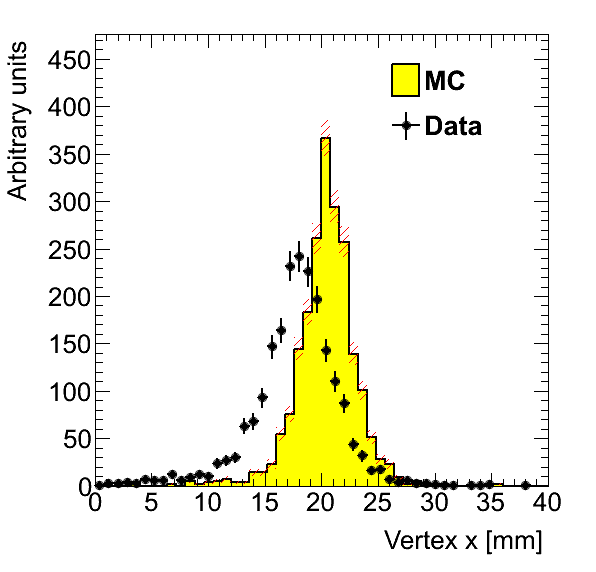
\includegraphics[ scale=0.25]{test2012/vertexing/figures/h_vtx_fr_y_h_vtx_y_dataMC_twotrksel.png}
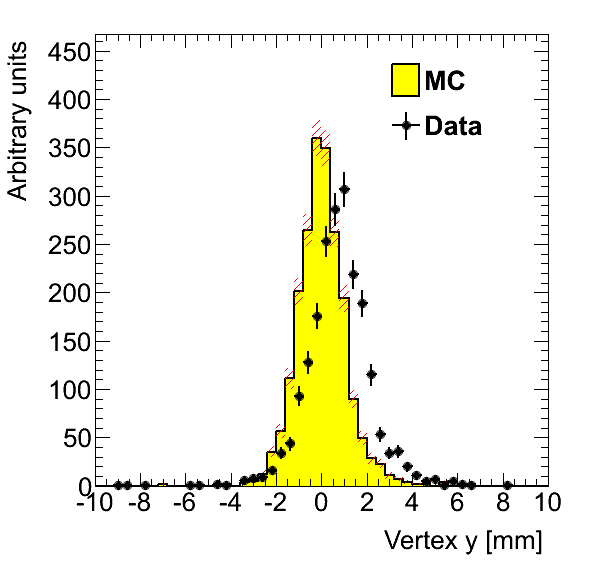
\includegraphics[ scale=0.25]{test2012/vertexing/figures/h_vtx_fr_z_h_vtx_z_dataMC_twotrksel.png}
\caption{\small{Vertex position represented by the distance of closest approach of the extrapolated momentum vectors upstream of the analyzing magnet. The overall shift from zero is due to a 30~mrad rotation of the SVT with respect to the beam line.}}\label{fig:vtx_pos}
\end{figure*}
